\documentclass[11pt, a4paper]{article}

\usepackage[utf8]{inputenc}
\usepackage[T1]{fontenc}
\usepackage[margin=2.5cm]{geometry}
\usepackage{amsmath, amssymb}
\usepackage{booktabs}
\usepackage{graphicx}
\usepackage{hyperref}
\usepackage{xcolor}
\usepackage{listings}
\usepackage{enumitem}
\usepackage{parskip}
\usepackage{microtype}
\usepackage{tikz}
\usetikzlibrary{shapes.geometric, arrows.meta, positioning, fit, backgrounds}

\hypersetup{
    colorlinks=true,
    linkcolor=blue!60!black,
    citecolor=blue!60!black,
    urlcolor=blue!60!black,
}

\lstset{
    basicstyle=\ttfamily\small,
    backgroundcolor=\color{gray!8},
    frame=single,
    framerule=0.4pt,
    rulecolor=\color{gray!40},
    breaklines=true,
    columns=fullflexible,
}

\title{\textbf{Portfolio RL Agent: Architecture Design}\\[0.5em]
       \large Trading Game for NSE/BSE Equity Markets}
\author{market-agent project}
\date{September 2026}

\begin{document}

\maketitle
\tableofcontents
\newpage

% ──────────────────────────────────────────────────────────────────────────────
\section{Game Rules Summary}

The trading game defines the environment in which the RL agent operates.
The rules constrain agent behaviour rather than being learned objectives.

\begin{enumerate}[leftmargin=*, label=\textbf{\arabic*.}]
    \item The player starts with a configurable amount of cash.
    \item Initial portfolio value equals the initial cash amount.
    \item The player may buy and sell equities on BSE or NSE.
    \item \textbf{T+2 settlement.} Proceeds from a sale move into \emph{reserved cash},
          which has the same monetary value as cash but cannot be used to fund
          purchases. After a 2-trading-day delay, reserved cash converts to
          spendable cash.
    \item Purchases are capped by available (spendable) cash.
    \item $V_\text{portfolio} = V_\text{stocks} + C_\text{cash} + C_\text{reserved}$.
    \item \textbf{Decision frequency.} Buy/sell decisions may only be made when
          exchanges are open, at most once every 15 minutes, or immediately upon
          the release of a news item.
    \item \textbf{Maximum holding period.} Any position held for more than 10 calendar
          days is force-sold by the environment at the prevailing market price.
    \item \textbf{Objective.} Continuously maximise total portfolio value.
\end{enumerate}

% ──────────────────────────────────────────────────────────────────────────────
\section{MDP Formulation}

\subsection{State Space}

At each decision step $t$ the agent observes a state $s_t$ composed of four
parts.

\paragraph{Per-stock market embedding $\mathbf{m}_i$.}
The pre-trained DualCNN maps recent daily and hourly OHLCV history for stock
$i$ to a 256-dimensional embedding. During the first training phase this
encoder is frozen; a second fine-tuning phase can update it end-to-end.

\paragraph{Per-stock position state $\mathbf{p}_i$.}
A 4-dimensional vector describing the agent's current exposure to stock $i$:
\[
    \mathbf{p}_i = \bigl(w_i^\text{held},\; d_i / 10,\; \mathrm{pnl}_i,\;
                         p_i^\text{entry} / p_i^\text{current}\bigr)
\]
where $w_i^\text{held}$ is the current portfolio weight, $d_i \in [0,10]$ is
the number of days held (normalised by the 10-day cap), $\mathrm{pnl}_i$ is
the unrealised return, and $p^\text{entry}/p^\text{current}$ encodes whether
the position is in profit or loss.

\paragraph{Per-stock news signal $\mathbf{n}_i$.}
A 3-dimensional vector of the most recent LLM-classified signal for stock $i$
from the \texttt{NewsMonitor} pipeline:
$(\text{sentiment},\, \text{severity},\, \text{hours\_since\_release})$.

\paragraph{Global portfolio state $\mathbf{g}$.}
A 3-dimensional vector:
\[
    \mathbf{g} = \bigl(C_\text{cash} / V_\text{portfolio},\;
                       C_\text{reserved} / V_\text{portfolio},\;
                       \tau_\text{reserved} / 2\bigr)
\]
where $\tau_\text{reserved}$ is the normalised time until the oldest reserved
cash tranche unlocks.

\subsection{Action Space}

The action is a target portfolio weight vector
$\mathbf{w} \in \Delta^{N+1}$, one weight per candidate stock plus a cash
weight, constrained to the probability simplex:
\[
    w_i \geq 0, \quad \sum_{i=0}^{N} w_i = 1.
\]
$w_0$ denotes the cash allocation; $w_1, \ldots, w_N$ denote allocations to
the $N$ candidate stocks. The simplex constraint is enforced by a masked
softmax: any stock with $d_i \geq 10$ has its logit set to $-\infty$ before
the softmax, making forced sells automatic and differentiable. This
formulation follows the continuous-weight portfolio action space introduced
in~\cite{jiang2017portfolio}.

\subsection{Candidate Universe}

At each step the full $5{,}000+$ stock universe is pre-filtered to the top
$N = 100$ stocks by current SwingPredictor score. This keeps the action space
fixed-size and computationally tractable while still allowing the agent to
express meaningful allocation choices.

\subsection{Reward}

The reward at step $t$ is the log portfolio return penalised for
turnover~\cite{almgren2001execution}:
\[
    r_t = \log\!\frac{V_{t+1}}{V_t} - \lambda \sum_{i=1}^{N}
          \bigl|w_i^{(t)} - w_i^{(t-1)}\bigr|
\]
where $\lambda$ is a transaction cost coefficient calibrated to Kite
brokerage rates. Using log returns makes the reward scale-invariant and
additive over an episode.

\subsection{Environment Transitions}

The environment enforces the following mechanics on every step, in order:

\begin{enumerate}[label=\roman*.]
    \item \textbf{Forced sells.} Any stock with $d_i \geq 10$ is sold at the
          opening price of the current bar; proceeds go to reserved cash.
    \item \textbf{T+2 unlock.} Reserved cash tranches whose 2-day delay has
          elapsed are moved to spendable cash.
    \item \textbf{Trade execution.} The delta between target weights
          $\mathbf{w}^{(t)}$ and current weights is computed. Sells execute
          first (freeing cash), then buys, all at the mid-price of the current
          15-min bar. Sale proceeds go to reserved cash.
    \item \textbf{Portfolio valuation.} $V_{t+1}$ is computed from the closing
          price of the bar using Rule~6.
    \item \textbf{Reward computation.} $r_t$ is calculated and the new state
          $s_{t+1}$ is assembled.
\end{enumerate}

% ──────────────────────────────────────────────────────────────────────────────
\section{Network Architecture}

\subsection{Overview}

The architecture has four stages: feature extraction, per-stock encoding,
cross-stock attention, and action/value heads. Figure~\ref{fig:arch} shows
the data flow.

\begin{figure}[ht]
\centering
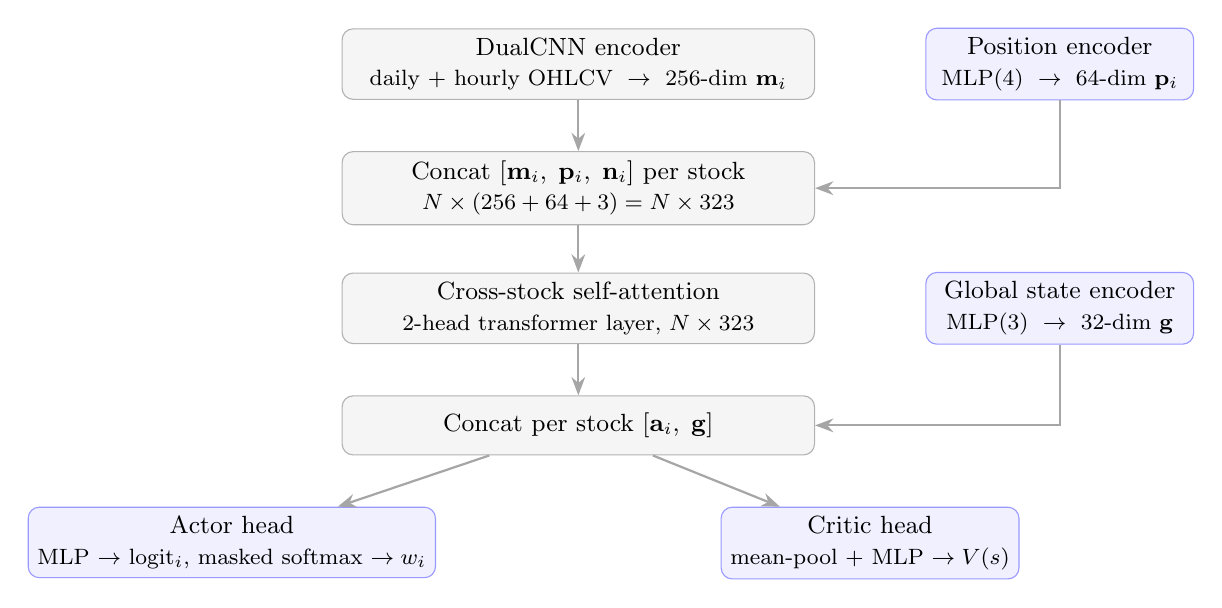
\begin{tikzpicture}[
    box/.style={rectangle, rounded corners=4pt, draw=gray!60, fill=gray!8,
                minimum width=6cm, minimum height=0.75cm,
                align=center, font=\small},
    side/.style={rectangle, rounded corners=4pt, draw=blue!40, fill=blue!6,
                 minimum width=3.4cm, minimum height=0.75cm,
                 align=center, font=\small},
    arr/.style={-Stealth, thick, color=gray!70},
    node distance=0.6cm
]

\node[box] (dualcnn)
    {DualCNN encoder\\
     {\footnotesize daily + hourly OHLCV $\;\to\;$ 256-dim $\mathbf{m}_i$}};

\node[side, right=1.4cm of dualcnn] (posenc)
    {Position encoder\\
     {\footnotesize MLP(4) $\;\to\;$ 64-dim $\mathbf{p}_i$}};

\node[box, below=0.65cm of dualcnn] (concat)
    {Concat $[\mathbf{m}_i,\;\mathbf{p}_i,\;\mathbf{n}_i]$ per stock\\
     {\footnotesize $N \times (256 + 64 + 3) = N \times 323$}};

\node[box, below=0.6cm of concat] (attn)
    {Cross-stock self-attention\\
     {\footnotesize 2-head transformer layer, $N \times 323$}};

\node[side, right=1.4cm of attn] (global)
    {Global state encoder\\
     {\footnotesize MLP(3) $\;\to\;$ 32-dim $\mathbf{g}$}};

\node[box, below=0.65cm of attn] (heads)
    {Concat per stock $[\mathbf{a}_i,\;\mathbf{g}]$};

\node[side, below left=0.65cm and -1.2cm of heads] (actor)
    {Actor head\\
     {\footnotesize MLP $\to$ logit$_i$, masked softmax $\to w_i$}};

\node[side, below right=0.65cm and -1.2cm of heads] (critic)
    {Critic head\\
     {\footnotesize mean-pool $+$ MLP $\to V(s)$}};

\draw[arr] (dualcnn)  -- (concat);
\draw[arr] (posenc.south) |- (concat.east);
\draw[arr] (concat)   -- (attn);
\draw[arr] (attn)     -- (heads);
\draw[arr] (global.south) |- (heads.east);
\draw[arr] (heads)    -- (actor);
\draw[arr] (heads)    -- (critic);

\end{tikzpicture}
\caption{Data flow through the policy and value networks. $\mathbf{a}_i$
         denotes the contextualised per-stock representation output by the
         self-attention layer.}
\label{fig:arch}
\end{figure}

\subsection{DualCNN Encoder (Frozen Phase)}

The existing \texttt{DualCNN\_v3} from \texttt{StockSwingPredictor} produces
a 256-dimensional market embedding $\mathbf{m}_i$ per stock from a 28-day
daily window and a 280-bar hourly window. Its weights are frozen during
initial RL training to avoid destroying the pre-trained price
representations.

\subsection{Position Encoder}

A two-layer MLP maps the 4-dimensional position state $\mathbf{p}_i$ to a
64-dimensional embedding. This gives the agent an explicit representation of
its current exposure to each stock, decoupled from the market signal.

\subsection{Cross-Stock Self-Attention}

After concatenating $[\mathbf{m}_i, \mathbf{p}_i, \mathbf{n}_i]$ for all $N$
candidate stocks, a single transformer encoder layer~\cite{vaswani2017attention}
with 2 attention heads produces contextualised per-stock representations.
This design is directly motivated by Relational Deep Reinforcement
Learning~\cite{zambaldi2018relational}, where self-attention allows an RL
agent to reason about relationships between entities in its observation —
here, the relative opportunity between stocks. It allows the agent to reason
about relative opportunities, e.g.\ rotating from a stock with high
unrealised gains into one with a stronger forward signal.

\subsection{Policy Head (Actor)}

For each stock $i$, the contextualised representation is concatenated with the
global state embedding $\mathbf{g}$ and passed through a small MLP to produce
a scalar logit $l_i$. A special cash logit $l_0$ is produced from $\mathbf{g}$
alone. The target weights are:
\[
    w_i = \frac{\exp(l_i) \cdot \mathbf{1}[d_i < 10]}
               {\sum_j \exp(l_j) \cdot \mathbf{1}[d_j < 10]}
\]
The mask $\mathbf{1}[d_i < 10]$ zeroes out stocks subject to forced sell
before normalisation, so the constraint from Rule~8 is satisfied by
construction.

\subsection{Value Head (Critic)}

The critic mean-pools the contextualised stock representations, concatenates
the global state $\mathbf{g}$, and passes the result through an MLP to
produce a scalar state value $V(s)$.

% ──────────────────────────────────────────────────────────────────────────────
\section{Training}

\subsection{Algorithm: Soft Actor-Critic (SAC)}

SAC~\cite{haarnoja2018sac, haarnoja2018sacapps} is chosen for three reasons:
\begin{itemize}
    \item \textbf{Off-policy.} A replay buffer allows multiple gradient updates
          per environment step, making historical data reuse efficient.
    \item \textbf{Continuous actions.} SAC handles continuous action spaces
          natively via reparameterisation.
    \item \textbf{Entropy regularisation.} The maximum entropy objective
          encourages portfolio diversification — the agent is penalised for
          collapsing all weight onto a single stock.
\end{itemize}

The SAC objective for the actor is:
\[
    \mathcal{L}_\pi = \mathbb{E}_{s \sim \mathcal{B}}\Bigl[
        \alpha \log \pi(\mathbf{w} \mid s) - Q(s, \mathbf{w})
    \Bigr]
\]
where $\alpha$ is a learned entropy temperature (tuned
automatically~\cite{haarnoja2018sacapps}) and $\mathcal{B}$ is the replay
buffer. PPO~\cite{schulman2017ppo} is retained as an on-policy baseline for
comparison.

\subsection{Episode Design}

Each training episode is a randomly sampled 6-month window from the historical
dataset (2010--2025), comprising approximately $6{,}000$ decision steps at
15-minute resolution. The environment is initialised with a configurable
starting cash value. Multiple episodes run in parallel on the historical
replay.

\subsection{Training Phases}

\begin{description}
    \item[Phase 1 --- Frozen encoder.]
        DualCNN weights are fixed. Only the position encoder, attention layer,
        and actor/critic heads are trained. This is faster per step and
        prevents destroying the pre-trained market representations early in
        training.
    \item[Phase 2 --- End-to-end fine-tuning.]
        All weights are unfrozen with a lower learning rate on the DualCNN
        layers. The policy signal can now shape the encoder towards
        portfolio-relevant features rather than swing-prediction features.
        Adversarial training~\cite{liang2018adversarial} may be added in this
        phase to improve robustness to distribution shift between historical
        training and live deployment.
\end{description}

\subsection{Replay Buffer}

A circular buffer stores transitions
$(s_t, \mathbf{w}_t, r_t, s_{t+1}, \mathrm{done}_t)$. Because the environment
is a deterministic historical replay, experience generation is fast and the
buffer can be seeded from many parallel episode workers before training begins.

% ──────────────────────────────────────────────────────────────────────────────
\section{Package Structure}

A new \texttt{TradingGame} package is added under \texttt{packages/}. It
depends on \texttt{StockSwingPredictor} (for the DualCNN and OHLCV cache) and
\texttt{NewsMonitor} (for news signals).

\begin{lstlisting}
packages/TradingGame/
+-- Project.toml
+-- src/
    +-- TradingGame.jl       # module entry, exports
    +-- types.jl             # Portfolio, TradingState, TradingAction,
    |                        # ReservedCashTranche, Episode, Transition
    +-- environment.jl       # step!, reset!, forced-sell, T+2 accounting
    +-- features.jl          # assemble state from InferenceCache + news
    +-- policy.jl            # position encoder, attention, actor/critic heads
    +-- sac.jl               # SAC update (actor loss, critic loss, alpha loss)
    +-- replay_buffer.jl     # circular buffer of Transition
    +-- backtest.jl          # run episode on historical data, return equity curve
    +-- display.jl           # Base.show overrides for Portfolio, Episode
\end{lstlisting}

\subsection{Package Dependency Rules}

\begin{center}
\begin{tabular}{ll}
    \toprule
    Package & Dependencies \\
    \midrule
    \texttt{TradingGame} & \texttt{StockSwingPredictor}, \texttt{NewsMonitor},
                           \texttt{Flux.jl} \\
    \texttt{StockSwingPredictor} & \texttt{TijoriData} \\
    \texttt{NewsMonitor} & (none within the project) \\
    \bottomrule
\end{tabular}
\end{center}

% ──────────────────────────────────────────────────────────────────────────────
\section{Pipeline Integration}

The full data-to-decision pipeline, integrating the new package with the
existing infrastructure, is as follows:

\begin{lstlisting}
# Morning setup
node sidecar/kite_login.js                    # fresh Kite session
julia scripts/update_ohlcv.jl --include-bse  # append yesterday's bars
julia scripts/build_cache.jl                 # rebuild InferenceCache

# Training (offline, run once / periodically)
julia --project=packages/TradingGame scripts/train_rl_agent.jl

# Live inference loop (during market hours)
julia --project=packages/TradingGame scripts/run_agent.jl
  -> every 15 min: assemble state from InferenceCache + live prices
  -> or on news:   NewsMonitor fires, agent re-evaluates immediately
  -> policy outputs target weights
  -> environment executes delta trades via Kite Connect orders API
\end{lstlisting}

% ──────────────────────────────────────────────────────────────────────────────
\section{Related Work}

\paragraph{Portfolio management with RL.}
The most direct precedent for this architecture is Jiang et al.\
\cite{jiang2017portfolio}, who frame portfolio management as an MDP with a
continuous simplex-constrained action space — the same formulation used here.
They apply an Exponential Gradient update and demonstrate that learning
directly over portfolio weights outperforms single-asset trading agents.
Liang et al.\ \cite{liang2018adversarial} extend this framework with
adversarial training to improve robustness to distribution shift between
training and deployment, which is directly relevant to the gap between our
historical backtesting environment and live market conditions. Liu et al.\
\cite{liu2021finrl} provide a comprehensive library and benchmarking
framework for portfolio RL that is useful for evaluating baselines.
The foundational objective of learning a trading policy via direct
reinforcement learning was established by Moody and Saffell~\cite{moody2001trading},
whose recurrent formulation underpins most subsequent work. Deng et
al.\ \cite{deng2017deep} combine CNNs for feature extraction with an RL
trading objective, foreshadowing the frozen-encoder approach taken here.

\paragraph{Attention in RL.}
The cross-stock self-attention layer is motivated by Relational Deep
Reinforcement Learning~\cite{zambaldi2018relational} (DeepMind), which
introduces multi-head self-attention inside an RL policy to allow the agent
to reason about pairwise relationships between entities in its observation.
The underlying attention mechanism is the scaled dot-product attention of
Vaswani et al.\ \cite{vaswani2017attention}.

\paragraph{SAC.}
The training algorithm is Soft Actor-Critic~\cite{haarnoja2018sac}, an
off-policy maximum-entropy actor-critic method for continuous action spaces.
The version with automatic entropy temperature tuning is used~\cite{haarnoja2018sacapps}.
PPO~\cite{schulman2017ppo} is included as an on-policy baseline.

\paragraph{Transaction costs.}
The turnover penalty in the reward function follows the optimal execution
framework of Almgren and Chriss~\cite{almgren2001execution}, the canonical
model for market impact and transaction cost penalties in portfolio
optimisation.

\paragraph{Deep RL for games.}
The broader context of applying deep networks as function approximators
in game-like sequential decision problems was established by DQN~\cite{mnih2015dqn},
then extended to superhuman performance in Go by AlphaGo~\cite{silver2016alphago}
and generalised across board games by AlphaZero~\cite{silver2018alphazero}.
While these systems address discrete-action, perfect-information settings,
they demonstrate the scalability of the deep RL paradigm that underpins
this architecture.

% ──────────────────────────────────────────────────────────────────────────────
\section{Open Questions}

\begin{enumerate}
    \item \textbf{Candidate universe size $N$.}
          $N = 100$ is the current proposal. A larger $N$ (e.g.\ 500) increases
          action space expressiveness but scales the attention layer as
          $O(N^2)$. This is the primary remaining architectural decision.

    \item \textbf{Transaction cost model.}
          Kite brokerage is flat Rs.\,20 per executed order for equity
          delivery. The turnover penalty $\lambda$ should be calibrated to
          reflect this in normalised return terms.

    \item \textbf{Dirichlet vs.\ softmax-Gaussian policy.}
          A Dirichlet distribution is the natural choice for simplex-constrained
          outputs and may produce better-calibrated uncertainty. Softmax of
          Gaussian logits is simpler to implement. Worth benchmarking both.

    \item \textbf{Order placement.}
          The \texttt{broker.jl} module currently reads portfolio state but
          does not place orders. Kite Connect order placement (market orders
          for live execution) needs to be added before live deployment.
\end{enumerate}

% ──────────────────────────────────────────────────────────────────────────────
\begin{thebibliography}{99}

\bibitem{almgren2001execution}
Almgren, R.\ and Chriss, N.\ (2001).
\newblock Optimal execution of portfolio transactions.
\newblock \textit{Journal of Risk}, 3(2):5--39.

\bibitem{deng2017deep}
Deng, Y., Bao, F., Kong, Y., Ren, Z., and Dai, Q.\ (2017).
\newblock Deep direct reinforcement learning for financial signal
  representation and trading.
\newblock \textit{IEEE Transactions on Neural Networks and Learning Systems},
  28(3):653--664.

\bibitem{haarnoja2018sac}
Haarnoja, T., Zhou, A., Abbeel, P., and Levine, S.\ (2018a).
\newblock Soft actor-critic: Off-policy maximum entropy deep reinforcement
  learning with a stochastic actor.
\newblock In \textit{Proceedings of the 35th International Conference on
  Machine Learning (ICML)}, pages 1861--1870.

\bibitem{haarnoja2018sacapps}
Haarnoja, T., Zhou, A., Hartikainen, K., Tucker, G., Ha, S., Tan, J.,
  Kumar, V., Zhu, H., Gupta, A., Abbeel, P., and Levine, S.\ (2018b).
\newblock Soft actor-critic algorithms and applications.
\newblock \textit{arXiv preprint arXiv:1812.05905}.

\bibitem{jiang2017portfolio}
Jiang, Z., Xu, D., and Liang, J.\ (2017).
\newblock A deep reinforcement learning framework for the financial portfolio
  management problem.
\newblock \textit{arXiv preprint arXiv:1706.10059}.

\bibitem{liang2018adversarial}
Liang, Z., Chen, H., Zhu, J., Jiang, K., and Li, Y.\ (2018).
\newblock Adversarial deep reinforcement learning in portfolio management.
\newblock \textit{arXiv preprint arXiv:1808.09940}.

\bibitem{liu2021finrl}
Liu, X., Rui, J., Gao, J., Yang, L., Yang, H., Zhu, M., Wang, C., Wang, Z.,
  and Guo, J.\ (2021).
\newblock {FinRL}: A deep reinforcement learning library for automated stock
  trading in quantitative finance.
\newblock In \textit{Proceedings of the Second ACM International Conference on
  AI in Finance (ICAIF)}.

\bibitem{mnih2015dqn}
Mnih, V., Kavukcuoglu, K., Silver, D., Rusu, A.~A., Veness, J., Bellemare,
  M.~G., Graves, A., Riedmiller, M., Fidjeland, A.~K., Ostrovski, G.,
  Petersen, S., Beattie, C., Sadik, A., Antonoglou, I., King, H., Kumaran, D.,
  Wierstra, D., Legg, S., and Hassabis, D.\ (2015).
\newblock Human-level control through deep reinforcement learning.
\newblock \textit{Nature}, 518(7540):529--533.

\bibitem{moody2001trading}
Moody, J.\ and Saffell, M.\ (2001).
\newblock Learning to trade via direct reinforcement.
\newblock \textit{IEEE Transactions on Neural Networks}, 12(4):875--889.

\bibitem{schulman2017ppo}
Schulman, J., Wolski, F., Dhariwal, P., Radford, A., and Klimov, O.\ (2017).
\newblock Proximal policy optimization algorithms.
\newblock \textit{arXiv preprint arXiv:1707.06347}.

\bibitem{silver2016alphago}
Silver, D., Huang, A., Maddison, C.~J., Guez, A., Sifre, L., van den
  Driessche, G., Schrittwieser, J., Antonoglou, I., Panneershelvam, V.,
  Lanctot, M., Dieleman, S., Grewe, D., Nham, J., Kalchbrenner, N., Sutskever,
  I., Lillicrap, T., Leach, M., Kavukcuoglu, K., Graepel, T., and Hassabis,
  D.\ (2016).
\newblock Mastering the game of {Go} with deep neural networks and tree search.
\newblock \textit{Nature}, 529(7587):484--489.

\bibitem{silver2018alphazero}
Silver, D., Hubert, T., Schrittwieser, J., Antonoglou, I., Lai, M., Guez, A.,
  Lanctot, M., Sifre, L., Kumaran, D., Graepel, T., Lillicrap, T.,
  Simonyan, K., and Hassabis, D.\ (2018).
\newblock A general reinforcement learning algorithm that masters chess, shogi,
  and {Go} through self-play.
\newblock \textit{Science}, 362(6419):1140--1144.

\bibitem{vaswani2017attention}
Vaswani, A., Shazeer, N., Parmar, N., Uszkoreit, J., Jones, L., Gomez,
  A.~N., Kaiser, {\L}., and Polosukhin, I.\ (2017).
\newblock Attention is all you need.
\newblock In \textit{Advances in Neural Information Processing Systems
  (NeurIPS)}, volume~30.

\bibitem{zambaldi2018relational}
Zambaldi, V., Raposo, D., Santoro, A., Bapst, V., Li, Y., Babuschkin, I.,
  Tuyls, K., Reichert, D., Lillicrap, T., Lockhart, E., Shanahan, M.,
  Langston, V., Pascanu, R., Botvinick, M., Vinyals, O., and Battaglia, P.\
  (2018).
\newblock Relational deep reinforcement learning.
\newblock \textit{arXiv preprint arXiv:1806.01830}.

\end{thebibliography}

\end{document}
